\documentclass{standalone}
\usepackage{graphicx}	
\usepackage{amssymb, amsmath}
\usepackage{color}

\usepackage{tikz}
\usetikzlibrary{intersections, backgrounds}
\usepackage{pgfmath}

\definecolor{light}{RGB}{220, 188, 188}
\definecolor{mid}{RGB}{185, 124, 124}
\definecolor{dark}{RGB}{143, 39, 39}
\definecolor{highlight}{RGB}{180, 31, 180}
\definecolor{gray10}{gray}{0.1}
\definecolor{gray20}{gray}{0.2}
\definecolor{gray30}{gray}{0.3}
\definecolor{gray40}{gray}{0.4}
\definecolor{gray60}{gray}{0.6}
\definecolor{gray70}{gray}{0.7}
\definecolor{gray80}{gray}{0.8}
\definecolor{gray90}{gray}{0.9}
\definecolor{gray95}{gray}{0.95}

\newcommand*{\offset}{0.025}

\begin{document}

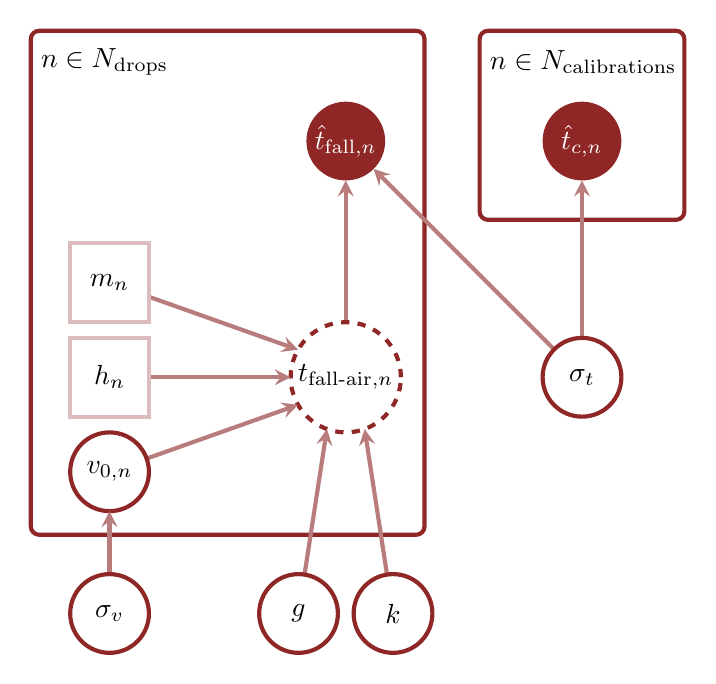
\begin{tikzpicture}[scale=0.4, thick]

\fill[white] (-10 - 0.1, 6.25 - 0.1) rectangle (10.75 + 0.1, 26 + 0.1);

\filldraw[fill=white, draw=dark, line width=1.5, rounded corners=3pt] (-10, 10) rectangle (2.5, 26);

\node[right] at (-10, 25) { $n \in N_{\text{drops}}$ };

\filldraw[fill=white, draw=dark, line width=1.5, rounded corners=3pt] (4.25, 20) rectangle (10.75, 26);

\node[right] at (4.25, 25) { $n \in N_{\text{calibrations}}$ };

\fill[color=dark] (0, 22.5) circle (1.25)
node[color=white] { $\hat{t}_{\mathrm{fall},n}$ };

\draw[->, >=stealth, color=mid, line width=1.5] (0, 15) -- (0, 22.5 - 1.25);

\filldraw[fill=white, draw=dark, dashed, line width=1.5] (0, 15) circle (1.75)
node[color=black] { $t_{\text{fall-air},n}$ };

\fill[color=dark] (7.5, 22.5) circle (1.25)
node[color=white] { $\hat{t}_{c, n}$ };

\draw[->, >=stealth, color=mid, line width=1.5] (7.5, 15) -- (7.5, 22.5 - 1.25);

\draw[->, >=stealth, color=mid, line width=1.5] (7.5, 15) -- ({0 + 1.25 * sin(45)}, {22.5 - 1.25 * sin(45)});

\filldraw[fill=white, draw=dark, line width=1.5] (7.5, 15) circle (1.25)
node[color=black] { $\sigma_{t}$ };

\draw[->, >=stealth, color=mid, line width=1.5] (-7.5, 15) -- (0 - 1.75, 15);

\filldraw[fill=white, draw=light, line width=1.5] (-7.5 - 1.25, 15 - 1.25) rectangle +(2.5, 2.5);
\node at (-7.5, 15) { $h_{n}$ };

\draw[->, >=stealth, color=mid, line width=1.5] (-7.5, 18) -- ({0 - 1.75 * cos(30)}, {15 + 1.75 * sin(30)});

\filldraw[fill=white, draw=light, line width=1.5] (-7.5 - 1.25, 18 - 1.25) rectangle +(2.5, 2.5);
\node at (-7.5, 18) { $m_{n}$ };

\draw[->, >=stealth, color=mid, line width=1.5] (-7.5, 12) -- ({0 - 1.75 * cos(30)}, {15 - 1.75 * sin(30)});

\filldraw[fill=white, draw=dark, line width=1.5] (-7.5, 12) circle (1.25)
node[color=black] { $v_{0, n}$ };

\draw[->, >=stealth, color=mid, line width=1.5] (-7.5, 7.5) -- (-7.5, 12 - 1.25);

\filldraw[fill=white, draw=dark, line width=1.5] (-7.5, 7.5) circle (1.25)
node[color=black] { $\sigma_{v}$ };

\draw[->, >=stealth, color=mid, line width=1.5] (-1.5, 7.5) -- ({0 - 1.75 * cos(70)}, {15 - 1.75 * sin(70)});

\filldraw[fill=white, draw=dark, line width=1.5] (-1.5, 7.5) circle (1.25)
node[color=black] { $g$ };

\draw[->, >=stealth, color=mid, line width=1.5] (1.5, 7.5) -- ({0 + 1.75 * cos(70)}, {15 - 1.75 * sin(70)});

\filldraw[fill=white, draw=dark, line width=1.5] (1.5, 7.5) circle (1.25)
node[color=black] { $k$ };

\end{tikzpicture}

\end{document}  